\section{Community dynamics of question answering}

\subsection{A reputation pyramid}

\subsection{The activity level of a question}
In the previous section, we illustrate the structure of users' reputation pyramid, which explains how answers arrival process relates to the user's reputation, as well as other phenomena from our observation. In this section, we would investigate more on voting, another significant mechanism of Stack Overflow. Except for merely answerers and questioners, other users can also involve in those QA sections by commenting, voting, etc.. The voting mechanism is not only applicable to answers but also to questions, and it is also considered as an important factor to reflect community involvement and evaluation. From our observation of Stack Overflow, we notice that questions with more answers are more likely to benefit from community involvement: answers will get higher votes and questions will receive more favorites. Highly active QA processes are more inclined to benefit from the community, instead of a competence among answerers themselves.  Based on our observation, our goal is to validate whether if the activity level is able to explain the feedback and evaluation from the community activities.

\textbf{Higher activity produces benefits.}
Like we discussed, unlike the features of general QA sites, Stack Overflow is programming-oriented, the questions are generally hard to be answered by majority community users. Furthermore, based on our observation from the previous section, answerers' arrival time is related to acceptance rate and answerers' reputation, it motivates answerers to answer a question quickly once it is posted. However, is there a competitive relationship existing among answerers?

%Fig6
%2010
\begin{figure}[!t]
	\centering
	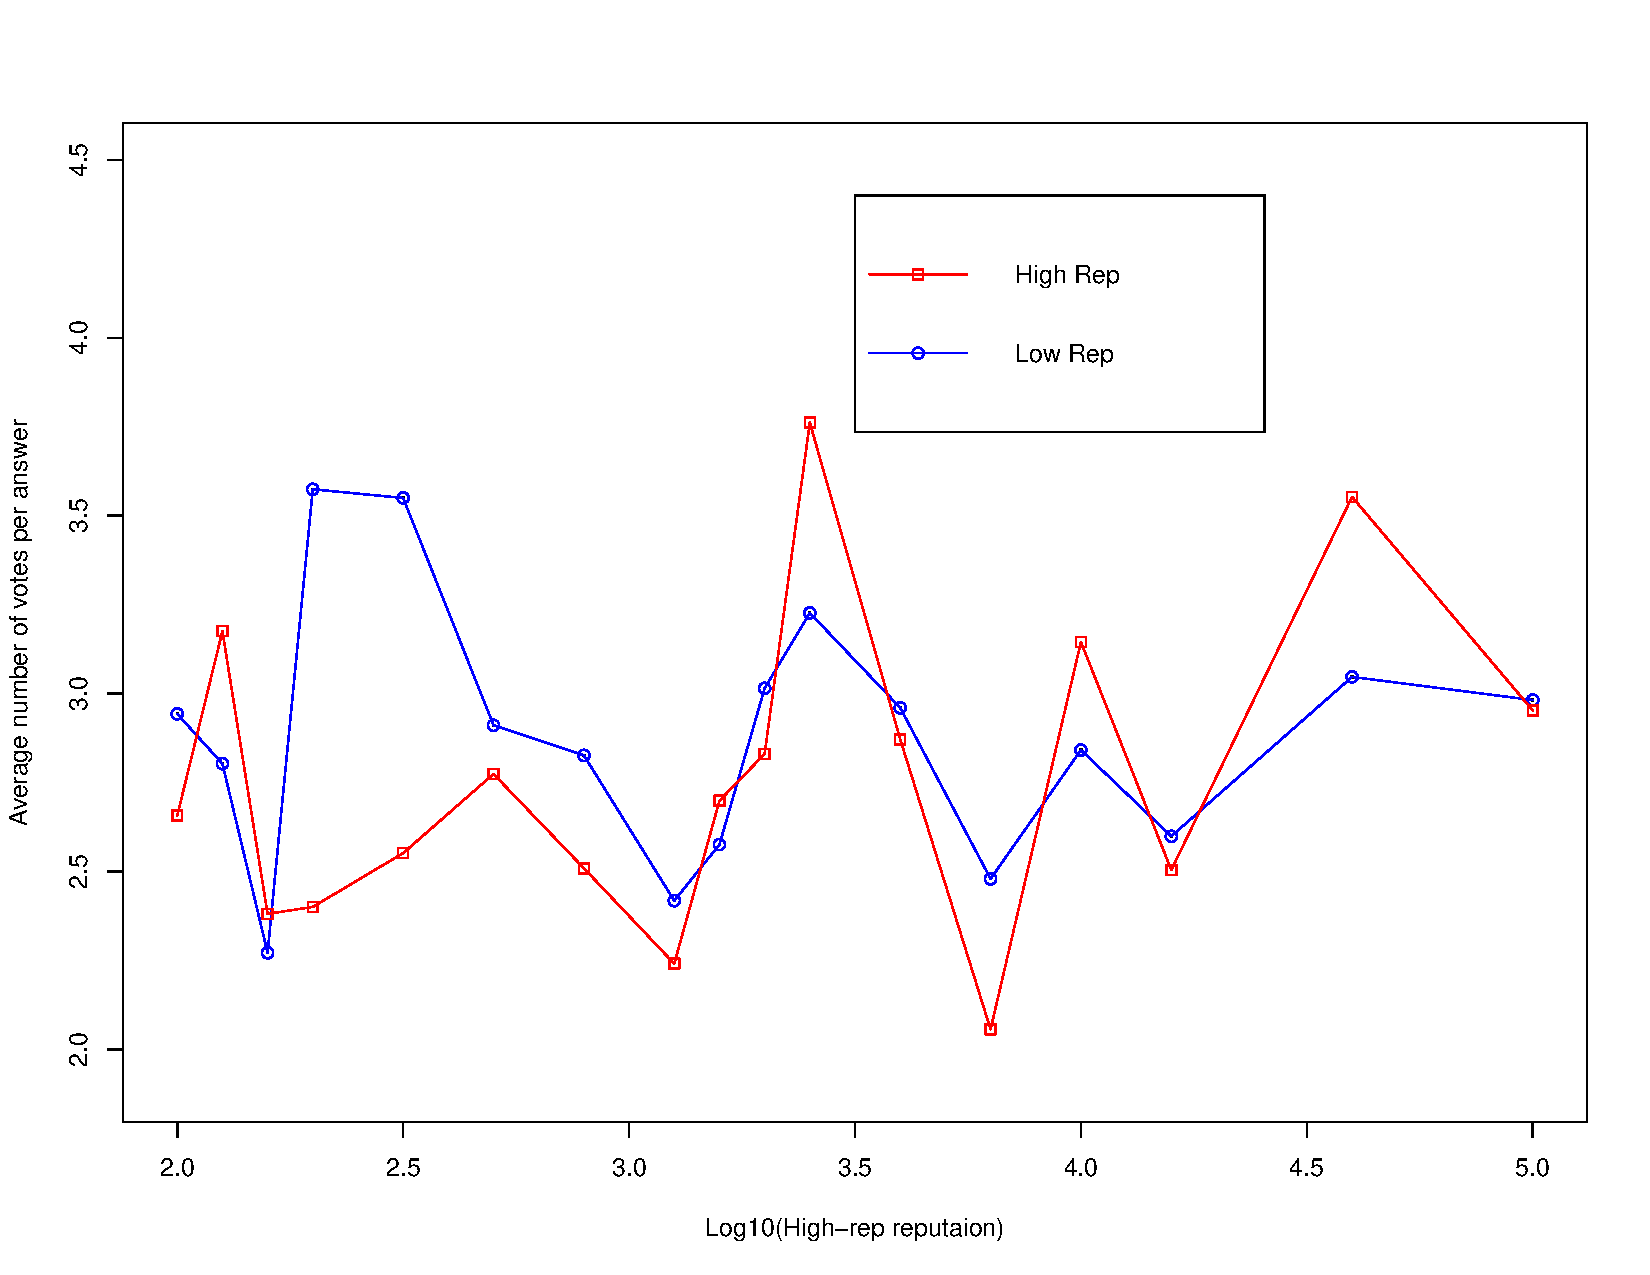
\includegraphics[width=0.8\columnwidth]{img/Fig6_2010.pdf}
	\caption{Fig 6 2010.}
	\label{fig:fig6_2010}
\end{figure}

\begin{figure}[!t]
	\centering
	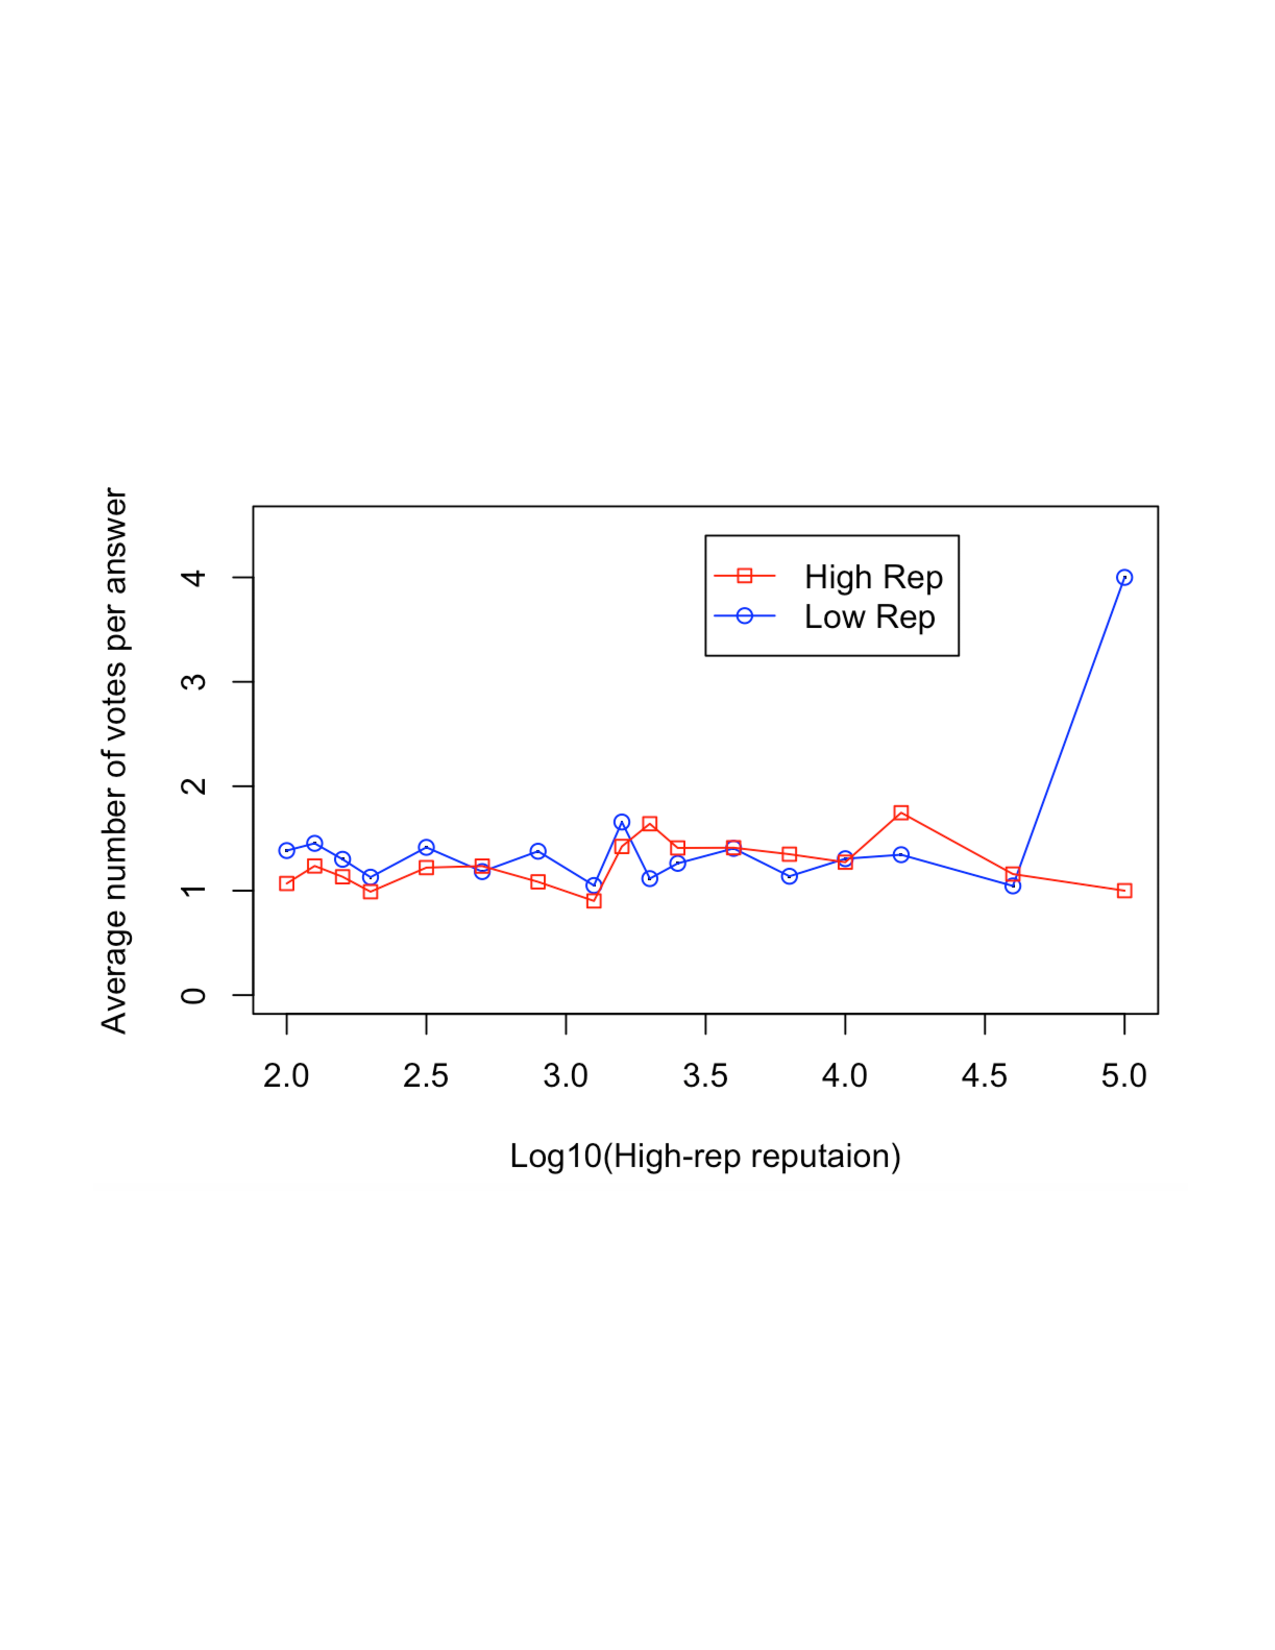
\includegraphics[width=0.8\columnwidth]{img/Fig6_2017.pdf}
	\caption{Fig 6 2017.}
	\label{fig:fig6_2017}
\end{figure}

In order to answer the question above, we choose all the questions with exactly two answers as our target dataset. Suppose $r_{i}$ is the reputation of the \textit{i}-th answerer, and $v_{i}$ is the number of vote score of the \textit{i}-th answer. If there exists a trend where $v_{1}$ goes up while $v_{2}$ decreases, we consider there's a competitive relationship between two answerers. Now we set the value of $r_{i}$ unchanged as x axis, and compare the average vote score for both answerers. To begin with, we collected data from all questions with two answers, and separate answers according to answerers' reputation. Since the dataset is highly biased, majority users have very limited reputation, which means they are either non-active users or possibly non-questioner or answerer. Adopting data from this part of users can deviate our result, we set a threshold where lower reputation users of the two answerers should have reputation between 75 and 125. In order to make the graph easier to interpret, first we scale x axis, which represents higher reputation users' reputation, using a logarithmic(base 10). For each reputation score, we use an average value to present higher and lower answerers' reputation respectively. Instead of representing vote score for each reputation point, we smooth the curve by splitting the vote scores into groups, according to different reputations in x axis, and calculate the average value of the group. From Fig\ref{fig:fig6_2010} we notice that in most cases, answer vote scores from high and low reputation users have similar trend, they either decrease or increase together, but high reputation answerers' answer votes have higher variance. The corresponding pattern reveals that in most cases, the two answerers do not have a competitive relationship. Similarly, this trend can also be noticed during 2015 to 2017. However, we notice the later dataset have relatively less average vote score, this could probably indicate that although there are a great amount of newly introduced answers, the quality of such answers are not as good as before, or the question has been sufficiently answered, newly added answers does not contribute much to the question. 


%Fig7
\begin{figure}[!t]
	\centering
	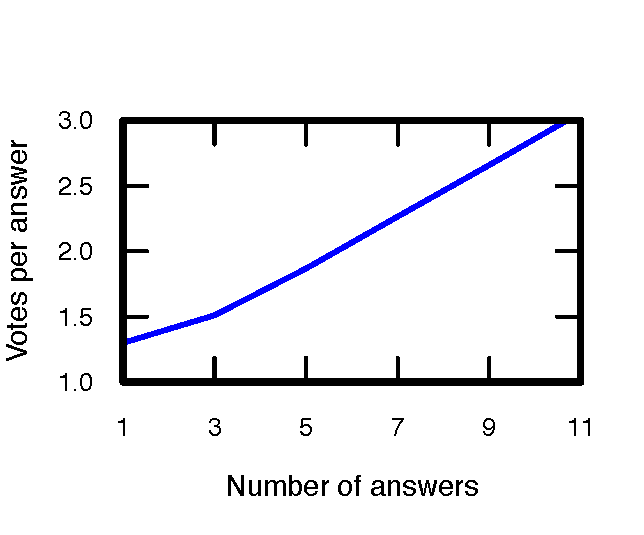
\includegraphics[width=0.8\columnwidth]{img/Fig7_2010.pdf}
	\caption{Fig 7 2010.}
	\label{fig:fig7_2010}
\end{figure}

\begin{figure}[!t]
	\centering
	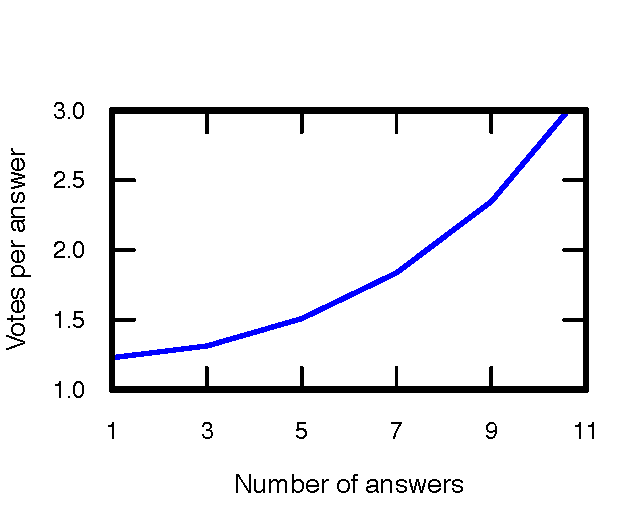
\includegraphics[width=0.8\columnwidth]{img/Fig7_2017.pdf}
	\caption{Fig 7 2017.}
	\label{fig:fig7_2017}
\end{figure}
In the following step, we aim to investigate the relationship between the number of answers in each question, to number of votes per answer. This work is to testify the correctness of the competition theory. If there exists competitive relationship among answers, we would expect a decreasing number of votes per answer, as the number of answers increases. From Fig \ref{fig:fig7_2010} we find that the average number of votes display an ascending trend as number of answers increases. This fact shows that the hotspot questions (questions with more answers) are more likely to benefit from community attention. 